\documentclass{article}
\usepackage{tikz}
\usepackage{pgfplots}
\usepackage{svg}
\usepackage{amsmath}
\usepackage{array}
\usepackage[skins]{tcolorbox}
\usepackage[version=4]{mhchem}
\usepackage[a4paper, total={6in, 9in}]{geometry}
\usepackage{fourier}
\usepackage{xymtex}
\usepackage{textcomp}
\usepackage{eurosym}
\usepackage{caption}
\usepackage{longtable}
\usepackage{float}
\usepackage{attachfile}
\usepackage{multirow}
\usepackage{amsfonts} 
\usepackage{tabularray}
\usepackage{colortbl}
\usepackage{xcolor}
\usepackage{graphicx}
\usepackage[table]{xcolor}
\UseTblrLibrary{booktabs}
\usepackage[bottom]{footmisc}
\pgfplotsset{compat=1.18}
\usepackage{siunitx}
\usepgfplotslibrary{colormaps}

\captionsetup[table]{name=Tabella}
%<\pagenumbering{gobble}

% Indice
\renewcommand*\contentsname{Indice}
\setcounter{tocdepth}{3}
%\setcounter{secnumdepth}{2}

%Tabellle
\usepackage{booktabs}
\usepackage{caption}
\usepackage{float}
\usepackage{titlesec}
\usepackage{capt-of}

%dashed line
\usepackage{array}
\usepackage{arydshln}
\setlength\dashlinedash{0.2pt}
\setlength\dashlinegap{1.5pt}
\setlength\arrayrulewidth{0.3pt}

%Widows & Orphans & Penalties

\widowpenalty500
\clubpenalty500
\clubpenalty=9996
\exhyphenpenalty=50 %for line-breaking at an explicit hyphen
\brokenpenalty=4991
\predisplaypenalty=10000
\postdisplaypenalty=1549
\displaywidowpenalty=1602
\floatingpenalty = 20000



%colori custom
\definecolor{myyellow}{RGB}{245, 215, 66} 
\definecolor{myred}{RGB}{255, 115, 69} 
\definecolor{mylightblue}{RGB}{134, 213, 247} 
\definecolor{myblue}{RGB}{93, 123, 186} 


\newtcolorbox{es}[2][]{%
	enhanced,colback=white,colframe=black,coltitle=black,
	sharp corners,boxrule=0.4pt,
	fonttitle=\itshape,
	attach boxed title to top left={yshift=-0.5\baselineskip-0.4pt,xshift=2mm},
	boxed title style={tile,size=minimal,left=0.5mm,right=0.5mm,
		colback=white,before upper=\strut},
	title=#2,#1
}


%sfondi colorati
\newcommand{\giallo}[1]{\colorbox{myyellow}{$\displaystyle #1$}}
\newcommand{\rosso}[1]{\colorbox{myred}{$\displaystyle #1$}}
\newcommand{\azzurro}[1]{\colorbox{mylightblue}{$\displaystyle #1$}}
\newcommand{\blu}[1]{\colorbox{myblue}{$\displaystyle #1$}}

\title{Relazione di laboratorio - Periodo di un pendolo semplice}
\author{Federico Cesari}
\date{Aprile 2024}




%%%%%%%%%%%%%%%%%%%%%%%%%%%%%%%%%%%%%%%%%%%%%%%%%%%%%%%%%
%%				INIZIO DOC
%%%%%%%%%%%%%%%%%%%%%%%%%%%%%%%%%%%%%%%%%%%%%%%%%%%%%%%%%


\begin{document}
	\begin{titlepage}
   \begin{center}
       \vspace*{1cm}
        
       \textbf{\LARGE Relazione di laboratorio - Esperienza di Poisson}
       
       \vspace{0.3cm}
       \large \textit{Rate di una sorgente radioattiva} \\
       
       \vspace{0.5cm}
       \Large Federico Cesari \\
       
       \small 1096759

			
		\vspace{1cm}
		\begin{center}
			\includegraphics[scale=1.2]{geiger.jpeg}	
		\end{center}
		
		

       \vfill
            
       
            
       \vspace{0.8cm}
     
       
            
       corso A\\
       Università degli studi di Torino, Torino\\
       3 marzo 2024\\
       
            
   \end{center}
\end{titlepage}

	\tableofcontents
	
	%\newpage
	%\textcolor{white}{.}
	%\vfill
	\newpage
	\section*{Scopo dell’esperienza e premesse teoriche}
	L'esperienza ha come obiettivi la misura del calore specifico \(c_{x}\) di un corpo metallico (un cilindro di acciaio) tramite l'utilizzo di un calorimetro e la taratura di quest'ultimo determinata dalla sua massa equivalente \(m_{e}\). \\
	
	\noindent
	Il principio zero della termodinamica afferma che tra due corpi a temperature differenti posti a contatto avviene uno scambio di calore che ne fa variare le temperature portandoli ad una temperatura di equilibrio. Inoltre la quantità di calore ceduto dal corpo caldo è uguale al calore assoribito da quello freddo:
	\[ 
	|Q_{\text{ced}}| = |Q_{\text{ass}}|
	\]
	con il calore espresso come \(Q = mc\Delta T\): prodotto di massa del corpo, il suo calore specifico e la sua variazione di temperatura. 
	
	Nel nostro caso il calore ceduto è quello del sistema del calorimetro (calorimetro + acqua). Con temperatura del sistema acqua (\(m_{a}\)) + calorimetro \(T_{1}\) e temperatura \(T_{2}\) del corpo (\(m_{c}\))  Si può riscrivere la prima equazione come:
	\begin{equation}\label{uno}
	\sum m_{\text{cal}}c_{\text{cal}}(T_{\text{eq}} - T_{1}) +  m_{a}c_{a}(T_{\text{eq}} - T_{1}) = m_{c}c_{x}(T_{2} - T_{\text{eq}})
	\end{equation}
	Durante l'esperieza verrà calcolata la massa equivalente \(m_{e}\), massa d'acqua che assorbe lo stesso calore che viene sottratto dal sistema calorimetro. Per farlo si versa nel calorimetro una massa \(m'_{a}\) d'acqua calda (di cui è noto il calore specifico), riscrivendo l'equilibrio energetico si può determinare \(m_{e}\)
	\[ 
	m'_{a}c_{a}(T'_{2} - T'_{\text{eq}}) = (m_{a} + m_{e})(T_{\text{eq}})
	\]
	 \[ 
	 m_{e}c_{a}(T'_{2} - T'_{\text{eq}}) +  m_{a}c_{a}(T'_{\text{eq}} - T'_{1}) = m_{a}c_{a}(T'_{\text{eq}} - T'_{1})
	\]
	 dove \(m_{e}\) è l'unica incognita. \\
	 
	
	 \noindent
	 Trovata la massa equivalente è possibile ricavare il calore specifico \(c_{x}\) del cilindro metallico sostituendo \(\sum m_{\text{cal}}c_{\text{cal}}\) con \(m_{e}c_{a}\) nella (\ref{uno}):
	 \[ 
	 m_{e}c_{a}(T_{\text{eq}} - T_{1}) +  m_{a}c_{a}(T_{\text{eq}} - T_{1}) = m_{c}c_{x}(T_{2} - T_{\text{eq}})
	 \]
	
	
	\section*{Strumentazione}
	\begin{table}[H] \centering
		%\ra{1.3}
		\begin{small}
			\begin{tabular}{@{}lcr@{}}\toprule
				\textbf{strumento}& \textbf{sensibilità}& \textbf{utilizzo} \\ \midrule
				\textbf{Cronometro digitale}	&	\(0.01 \SI{}{\second}\) s &  misura tempo presa dati\\  \hdashline
				\textbf{Termometro a mercurio (1)}	& \(0.01 ^\circ C\)	 &  misura temperatura acqua nel calorimetro\\  \hdashline
				\textbf{Termometro a mercurio (2)}	& \(1 ^\circ C\)	 & misura temperatura ambiente  \\  \hdashline
				\textbf{Termometro digitale}	& \(0.01 ^\circ C\)	 &  misura temperatura acqua calda nella borraccia (\(m'_{a}\))\\  \hdashline
				\textbf{ilancia elettronica} & \(0.0001 \SI{}{\kilogram}\) & misura masse \\ \bottomrule
			\end{tabular}
		\end{small}
		\caption{Misure preliminari (masse)}
	\end{table}
	Ovviamente è stato utilizzato un calorimetro e un bollitore per scaldare l'acqua (e il corpo a bagnomaria).
	
	\newpage
	\section{Prima presa dati}
	\subsection{Cilindro metallico}
	Per prima cosa si procede all'acquisizioni di alcune misure preliminari. Alcune di queste saranno già utilizzabili per il calcolo finale del calore specifico del cilindro metallico, altre invece verranno utilizzate per ricavare altri dati utili. Pesiamo sulla bilancia il vaso del calorimetro, il vaso con all'interno circa \(2.6 \SI{}{\kilogram}\) d'acqua, il cilindro metallico e il becher (nel caso sia necessario tarare qualche misura succesivamente).
	
	L'acqua versata all'interno del vaso è stata diluita con acqua fredda fino a farla arrivare ad una temperatura di circa \(14 ^\circ C\), in modo da reintrare nella scala di lettura del termometro fissato nel calorimetro (\(12-24 ^\circ C\)).
	
	Una volta versata, viene registrata la temperatura dell'acqua a intervalli di un minuto per quasi quindici minuti.
	
	Si immerge il cilindro metallico in un bollitore per scaldarlo fino a una temperatura di circa \(90 ^\circ C\). Subito prima dell'immersione del cilindro nel vaso pieno d'acqua si acquisiscono le temperature dell'acqua nel vaso, del corpo e dell'ambiente così da correggere eventuali dispersioni avvenute nell'attesa che il cilindro si scaldasse.
	
	\vspace{1cm}
	\begin{minipage}{0.4\textwidth}
		\begin{table}[H] \centering
			%\ra{1.3}
			\begin{small}
				\begin{tabular}{@{}lrr@{}}\toprule
					\textbf{Oggetto}& &  \(\boldsymbol{(m \pm 0.0001) \SI{}{\kilogram}}\) \\ \midrule
					\textbf{Massa vaso}	&	 & \(1.3775\)   \\  \hdashline
					\textbf{Massa vaso + acqua}	&	 & \(3.9825\)   \\  \hdashline
					\textbf{Massa corpo}	& \(m_{c}\)	 & \(0.3866\)   \\  \hdashline
					\textbf{Massa becher}	&	 & \(0.2246\)   \\
					\bottomrule
				\end{tabular}
			\end{small}
			\caption{Misure preliminari (masse)}
		\end{table}
	\end{minipage}
	\begin{minipage}{0.6\textwidth}
		\begin{table}[H] \centering
			%\ra{1.3}
			\begin{small}
				\begin{tabular}{@{}lrr@{}}\toprule
					\textbf{Oggetto}					&  			& \textbf{(\(\boldsymbol{T}\))} \(\boldsymbol{^\circ C}\))\\ \midrule
					\textbf{Temp. cilindro metallico}	& 	\(T_{2}\)		& \(86 \pm 1\)	 \\  \hdashline
					\textbf{Temp. acqua}				&					&\(15.20 \pm 0.01\)		 	 \\  \hdashline
					\textbf{Temp. ambiente}				&					& \(19 \pm 1\)		 	  \\  
					\bottomrule
				\end{tabular}
			\end{small}
			\caption{Misure preliminari (temperature)}
		\end{table}
	\end{minipage}
	\vspace{1cm}
	
	
	Dalle seguenti misure si ricava la massa d'acqua \(m_{a}\) presente nel calorimetro come divverenza della massa del vaso più l'acqua e la massa del vaso: \(\boldsymbol{(m_{a} = 2.6050\pm 0.0002)\SI{}{\kilogram}}\)\footnotemark. \\


	\noindent
	Immergo il cilindro metallico nell'acqua del calorimetro si acquisisce la temperatura dell'acqua a intervalli di \(5 s\) fino a che questa non raggiuge una soglia di equilibrio. Una volta raggiunta la temperatura di equilibrio si acquisisce nuovamente a intervalli di un minuto.
	
	
	\begin{center}
		\begin{figure}[H]
			\centering
			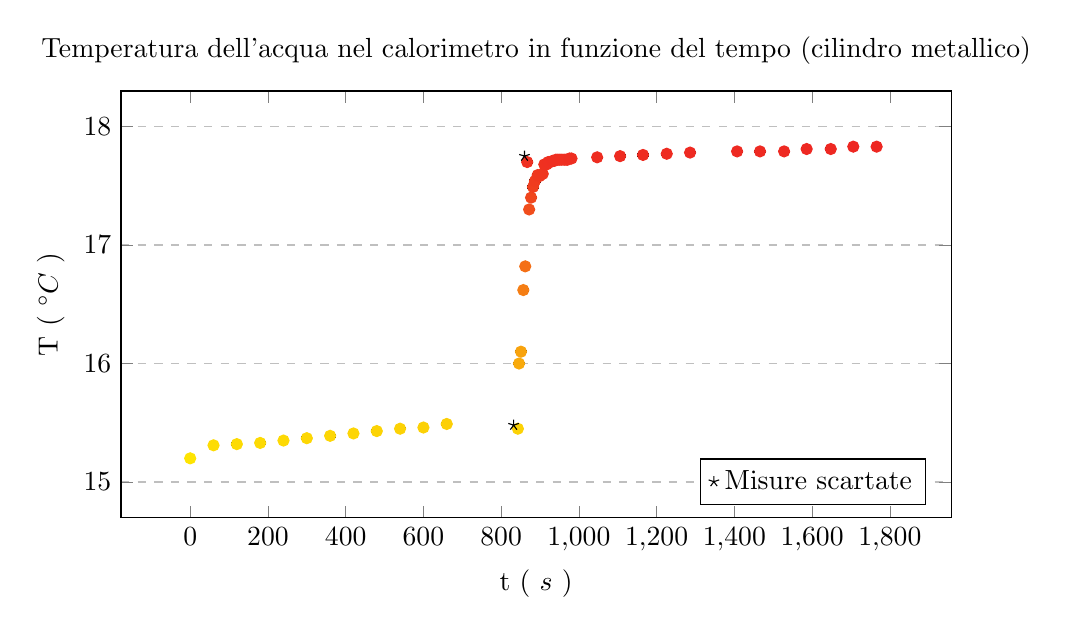
\begin{tikzpicture}
				\begin{axis}[
					title={Temperatura dell'acqua nel calorimetro in funzione del tempo (cilindro metallico)},
					xlabel={t ( $s$ )},
					ylabel={T ( $^\circ C$ )},
					xmin=0, xmax=1780,
					ymin=15, ymax=18,
					xtick={},
					ytick={},
					legend pos=south east,
					ymajorgrids=true,
					grid style=dashed,
					enlargelimits=0.1,
					width=\textwidth,
					height=7cm,
					point meta min=15,
					point meta max=18,
					colormap={yellowred}{
						color(0cm)=(yellow)
						color(1cm)=(red)
					},
					]
					
					% Define the data
					\pgfplotstableread{
						x y yerr
						0 15.2 0.01
						60 15.31 0.01
						120 15.32 0.01
						180 15.33 0.01
						240 15.35 0.01
						300 15.37 0.01
						360 15.39 0.01
						420 15.41 0.01
						480 15.43 0.01
						540 15.45 0.01
						600 15.46 0.01
						660 15.49 0.01
						843 15.45 0.01
						846 16.0 0.01
						851 16.1 0.01
						857 16.62 0.01
						862 16.82 0.01
						867 17.7 0.01
						872 17.3 0.01
						877 17.4 0.01
						882 17.49 0.01
						887 17.54 0.01
						894 17.59 0.01
						898 17.58 0.01
						901 17.59 0.01
						907 17.6 0.01
						911 17.68 0.01
						917 17.68 0.01
						921 17.7 0.01
						927 17.7 0.01
						932 17.71 0.01
						937 17.71 0.01
						941 17.72 0.01
						946 17.72 0.01
						951 17.72 0.01
						956 17.72 0.01
						962 17.72 0.01
						967 17.72 0.01
						971 17.72 0.01
						976 17.73 0.01
						981 17.73 0.01
						1047 17.74 0.01
						1106 17.75 0.01
						1165 17.76 0.01
						1226 17.77 0.01
						1286 17.78 0.01
						1407 17.79 0.01
						1466 17.79 0.01
						1528 17.79 0.01
						1586 17.81 0.01
						1648 17.81 0.01
						1706 17.83 0.01
						1766 17.83 0.01
					} \datatable
					
					% Plot the data with gradient
					\addplot[
					scatter, 
					only marks, 
					scatter src=explicit,
					scatter/use mapped color={
						draw=mapped color,
						fill=mapped color
					},
					error bars/.cd,
					y dir=both, y explicit
					]
					table[x=x, y=y, y error=yerr, meta=y] {\datatable};
					\addplot[
					only marks,
					mark=star,
					]
					coordinates {(832, 15.48)};
					\addplot[
					only marks,
					mark=star,
					]
					coordinates {(860, 17.75)};
					\legend{,,Misure scartate}
				\end{axis}
			\end{tikzpicture}
		\end{figure}
	\end{center}
	
	Analizzando la presa dati complessiva sono evidenti due sbavature, dovute a un errore di battitura o di lettura sul termometro, che vado a scartare. E' chiaro che la prima imprecisione (temperatura misurata nell'istante di immersione del cilindro) è sicuramente sbagliata: la temperatura dell'acqua stava aumentando gradualmente e non è fisicamente spiegabile un crollo simile. Anche la seconda esce completamente fuori dall'andamento della temperatura in quegli istanti ed è quindi ragionevole scartarla. \\
	
	\noindent
	Avendo dovuto scartare la temperatura all'istante di immersione si dovrà ricavare \(T_{1}\) temperatura iniziale dell'acqua tramite un fit lineare delle prime misure; nello stesso modo si determinerà \(T_{\text{eq}}\) temperatura di equilibrio.
	
	\subsubsection{Fit lineare \(T_{1}\) e \(T_{\text{eq}}\)}
	Per ricavare \(T_{\text{eq}}\) si traccia  la retta di best fit delle temperature finali e la si interseca con la retta \(x=t_{i}\) tempo di immersione del corpo. Si andrà quindi a simulare un "innalzamento istantaneo" della temperatura. 
	
	Risulta molto più semplice traslare il grafico, come riportato sotto, portando \(t_{i} = 843 s\) sullo \(0\) (\(t' = t - 843s\)) così che le due temperature trovate abbiano come errore quello sull'intercetta \(b\). In appendice viene esposto un secondo metodo che non necessita la traslazione del grafico e in cui entra in gioco la covarianza (\ref{covarianza}). \\
	
	\noindent
	Per prima cosa troviamo \(T_{1}\):
	
	\begin{center}
		\begin{figure}[H]
			\centering
			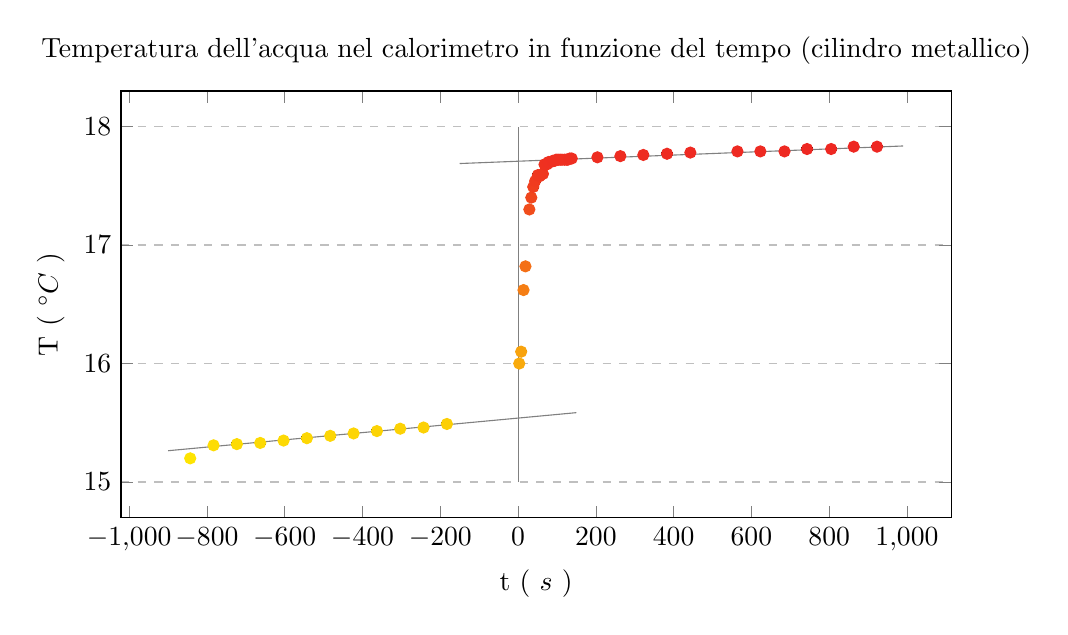
\begin{tikzpicture}
				\begin{axis}[
					title={Temperatura dell'acqua nel calorimetro in funzione del tempo (cilindro metallico)},
					xlabel={t ( $s$ )},
					ylabel={T ( $^\circ C$ )},
					xmin=-843, xmax=936,
					ymin=15, ymax=18,
					xtick={},
					ytick={},
					legend pos=south east,
					ymajorgrids=true,
					grid style=dashed,
					enlargelimits=0.1,
					width=\textwidth,
					height=7cm,
					point meta min=15,
					point meta max=18,
					colormap={yellowred}{
						color(0cm)=(yellow)
						color(1cm)=(red)
					},
					]
					
					% Define the data
					\pgfplotstableread{
						x y yerr
						-843 15.2 0.01
						-783 15.31 0.01
						-723 15.32 0.01
						-663 15.33 0.01
						-603 15.35 0.01
						-543 15.37 0.01
						-483 15.39 0.01
						-423 15.41 0.01
						-363 15.43 0.01
						-303 15.45 0.01
						-243 15.46 0.01
						-183 15.49 0.01
						3 16.0 0.01
						8 16.1 0.01
						14 16.62 0.01
						19 16.82 0.01
						29 17.3 0.01
						34 17.4 0.01
						39 17.49 0.01
						44 17.54 0.01
						51 17.59 0.01
						55 17.58 0.01
						58 17.59 0.01
						64 17.6 0.01
						68 17.68 0.01
						74 17.68 0.01
						78 17.7 0.01
						84 17.7 0.01
						89 17.71 0.01
						94 17.71 0.01
						98 17.72 0.01
						103 17.72 0.01
						108 17.72 0.01
						113 17.72 0.01
						119 17.72 0.01
						124 17.72 0.01
						128 17.72 0.01
						133 17.73 0.01
						138 17.73 0.01
						204 17.74 0.01
						263 17.75 0.01
						322 17.76 0.01
						383 17.77 0.01
						443 17.78 0.01
						564 17.79 0.01
						623 17.79 0.01
						685 17.79 0.01
						743 17.81 0.01
						805 17.81 0.01
						863 17.83 0.01
						923 17.83 0.01
					} \datatable
					
					% Plot the data with gradient
					\addplot[
					scatter, 
					only marks, 
					scatter src=explicit,
					scatter/use mapped color={
						draw=mapped color,
						fill=mapped color
					},
					error bars/.cd,
					y dir=both, y explicit
					]
					table[x=x, y=y, y error=yerr, meta=y] {\datatable};
					% Add vertical line at x=0
					\addplot [
					domain=15:18,
					samples=2,
					color=gray,
					]
					coordinates {(0,15) (0,18)};
					
					% Add line y = 15.539645 + 0.000306x
					\addplot [
					domain=-900:150,
					samples=100,
					color=gray,
					]
					{15.539645 + 0.000306*x};
					
					% Add line y = 17.707 + 0.00013x
					\addplot [
					domain=-150:990,
					samples=100,
					color=gray,
					]
					{17.707 + 0.00013*x};
				\end{axis}
			\end{tikzpicture}
		\end{figure}
	\end{center}
	\vspace{-1cm}
	\begin{minipage}{0.3\textwidth}
		\begin{table}[H]
			\centering
			\begin{tabular}{@{}cc@{}}
				\multicolumn{2}{c}{$\mathbf{T_{1}}$} \\ \midrule
			 	$\boldsymbol{t(s)}$ & $\boldsymbol{(T \pm 0.01) ^\circ C}$  \\ \midrule
				-783	& 	$15.31$   \\\hdashline
				-723	& 	$15.32$  \\\hdashline
				-663	& 	$15.33$  \\\hdashline
				-603	& 	$15.35 $   \\\hdashline
				-543	& 	$15.37$  \\\hdashline
				-483	& 	$15.39$   \\\hdashline
				-423	& 	$15.41 $   \\\hdashline
				-363	& 	$15.43 $   \\\hdashline
				-303	& 	$15.45 $   \\\hdashline
				-243	& 	$15.46$   \\ \hdashline
				-183	& 	$15.49 $  \\ \bottomrule   
			\end{tabular}
		\end{table}
	\end{minipage}
	\begin{minipage}{0.7\textwidth}
		Per trovare l'equazione della retta si utilizza il metodo dei minimi quadrati. L'errore relativo sul tempo è di due ordini di grandezza minore rispetto all'errore relativo sulla temperatura quindi quest'ultima sarà la variabile \(y\) e il tempo, che abbiamo appurato avere errore trascurabile rispetto a quello sulla temperatura, la \(x\). Con il metodo dei minimi quadrati si trovano i parametri \(\boldsymbol{a}\) e \(\boldsymbol{b}\) della retta:
		\[ 
		y = \boldsymbol{a} + \boldsymbol{b} x
		\]
		\[ 
		\boldsymbol{a = 15.28 \pm 0.01} \qquad \qquad \boldsymbol{b = 0.00031 \pm 0.00002}
		\]
		

		Per verificare che la retta trovata si adatti bene ai dati è bene effettuare un test del \(\chi^2\).
	\end{minipage}
	
	\paragraph{Ipotesi nulla} La retta \(y = \boldsymbol{a} + \boldsymbol{b}x\) descrive bene l’andamento dei dati osservati sperimentalmente.
	
	
	\begin{table}[H] \centering
		%\ra{1.3}
		\begin{small}
			\begin{tabular}{@{}lcr@{}}\toprule
				\multicolumn{3}{c}{\textbf{valori per test} \(\boldsymbol{\chi^2}\)}\\ \midrule
				\textbf{Livello di significatività}		 &  \(\alpha\) &\(0.05\)\footnotemark \\  \hdashline
					\textbf{Gradi di libertà}		 & \(n\)  &\((11-2) = 9\) \\   \hdashline
				\textbf{Valore di} \(\boldsymbol{\chi^2}\)	 & \(\chi^2\)  &\(2.61\)\\  \hdashline
				\(\boldsymbol{\chi^2}\) \textbf{sospetto}		& \(\chi^2_{\text{sos}}\)  &\(3.32\)\\ \hdashline
				\(\boldsymbol{\chi^2}\) \textbf{critico}		& \(\chi^2_{\text{cri}}\)  &\(16.91\)\\ 
				\bottomrule
			\end{tabular}
		\end{small}
		\caption{\(\chi^2\) \(T_{1}\)}
	\end{table}
	
	\noindent
	Il valore \(\chi^2\) rilevato è minore di quello sospetto: un piccolo valore di \(\chi^2\) è indice di barre d'errore troppo grandi o di una forte vicinanza tra valori sperimentali e valori teorici. A corroborare l'ipotesi di una presa dati molto precisa si rileva un coefficiente di correlazione lineare \(r = 0.997\). Inoltre l'errore associato alla temperatura (\(0.01 ^\circ C\)) è la sensibilità del termometro utilizzato e quindi non può essere stato sovrastimato. Concludo quindi accettando l'ipotesi nulla con un livello di significatività del 5\%.
	
	\subsubsection{Fit lineare \(T_{\text{eq}}\)}
	
	\begin{minipage}{0.7\textwidth}
		Per trovare l'equazione della retta si utilizza nuovamente il metodo dei minimi quadrati con il quale si ottengono i parametri \(\boldsymbol{a}\) e \(\boldsymbol{b}\) della retta:
		\[ 
		y = \boldsymbol{a} + \boldsymbol{b} x
		\]
		\[ 
		\boldsymbol{a = 17.71 \pm	0.02} \qquad \qquad \boldsymbol{b = 0.00013	\pm 0.00003}
		\]
		
		
		Per verificare che la retta trovata si adatti bene ai dati è bene effettuare un test del \(\chi^2\).
	\end{minipage}
	\begin{minipage}{0.3\textwidth}
		\begin{table}[H]
			\centering
			\begin{tabular}{@{}cc@{}}
				\multicolumn{2}{c}{$\mathbf{T_{\text{eq}}}$} \\ \midrule
				$\boldsymbol{t(s)}$ & $\boldsymbol{(T \pm 0.01) ^\circ C}$  \\ \midrule
				564	& 	$17.78$   \\\hdashline
				623	& 	$17.79$  \\\hdashline
				685	& 	$17.79$  \\\hdashline
				743	& 	$17.79$   \\\hdashline
				805	& 	$17.81$  \\\hdashline
				863	& 	$17.81$   \\\hdashline
				923	& 	$17.83$   \\ \bottomrule   
			\end{tabular}
		\end{table}
	\end{minipage}
	
	\paragraph{Ipotesi nulla} La retta \(y = \boldsymbol{a} + \boldsymbol{b}x\) descrive bene l’andamento dei dati osservati sperimentalmente.
	
	
	\begin{table}[H] \centering
		%\ra{1.3}
		\begin{small}
			\begin{tabular}{@{}lcr@{}}\toprule
				\multicolumn{3}{c}{\textbf{valori per test} \(\boldsymbol{\chi^2}\)}\\ \midrule
				\textbf{Livello di significatività}		 &  \(\alpha\) &\(0.05\)\footnotemark \\  \hdashline
				\textbf{Gradi di libertà}		 & \(n\)  &\((7-2) = 5\) \\   \hdashline
				\textbf{Valore di} \(\boldsymbol{\chi^2}\)	 & \(\chi^2\)  &\(2.24\)\\  \hdashline
				\(\boldsymbol{\chi^2}\) \textbf{sospetto}		& \(\chi^2_{\text{sos}}\)  &\(1.15\)\\ \hdashline
				\(\boldsymbol{\chi^2}\) \textbf{critico}		& \(\chi^2_{\text{cri}}\)  &\(11.07\)\\ 
				\bottomrule
			\end{tabular}
		\end{small}
		\caption{\(\chi^2\) \(T_{\text{eq}}\)}
	\end{table}
	
	\noindent
	Il valore \(\chi^2\) rilevato è compreso tra quello sospetto e quello critico quindi si conclude che, con livello di significatività del 5\%, la retta trovata descrive bene l'andamento dei  dati.
	
	
	\begin{es}{\(T_{1}\) e \(T_{\text{eq}}\)}
		Appurato che entrambe le rette possono essere buone approssimazioni dei miei dati, avendo traslato il grafico della temperatura portando il tempo di immersione sullo 0, le due temperature saranno semplicemente i due termini noti delle due rette:
		\[ 
		\giallo{\boldsymbol{T_{1} = 15.28	\pm 0.01}}\qquad \qquad \rosso{\boldsymbol{T_{\text{eq}} = 17.71	\pm 0.02}}
		\]
	\end{es}
	
	
	
	\subsection{Massa d'acqua}
	Per ricavare il valore della capacità termica del calorimetro si può calcolare la massa equivalente d'acqua, infatti vale \(C_{c} = m_{e} c_{a}\): la capacità termica del calorimetro è uguale al prodotto tra la massa equivalnte d'acqua e il calore specifico dell'acqua (quatità nota). \\
	
	\noindent
	Riprendeno l'equazione di equilibrio energetico possiamo ricavare la formula della massa equivalente, l'unica differenza è che questa volta non verrà utilizzato il cilindro metallico, ma bensì una massa d'ac	ua \(m'_{a}\) a temperatura \(T'_{2}\), così che sia noto il calore specifico del corpo immerso nel calorimetro con all'interno la massa \(m_{a(2)}\)\footnote{Il calcolo di \(m_{a(2)}\) è specificato nella fase finale della presa dati (\ref{calcolo me e cx})} d'acqua a temperatura \(T'_{1}\).
	
	\[ 
	 m'_{a}c_{x}(T'_{2} - T'_{e}) = (m_{e}c_{a} + m_{a(2)}c_{a})(T'_{\text{eq}} - T'_{1})
	\] 
	
	\[ 
	\to \quad m_{e} = \frac{m'_{a}(T'_{2} - T'_{\text{eq}})}{T'_{\text{eq}}-T'_{1}}
	\]
	
	\noindent
	Prima di tutto alcune misure preliminari: vengono pesate nuovamente tutte le masse (per eventuali residui di acqua rimasti sul cilindro o nei contenitori utilizzati per pesare) e misurate le temperature dell'acqua nel calorimetro e dell'acqua riscaldata nel bollitore.
	
	\vspace{1cm}
	\begin{minipage}{0.4\textwidth}
		\begin{table}[H] \centering
			%\ra{1.3}
			\begin{small}
				\begin{tabular}{@{}lrr@{}}\toprule
					\textbf{Oggetto}&  & \(\boldsymbol{(m \pm 0.0001) \SI{}{\kilogram}}\) \\ \midrule
					\textbf{Massa becher}	&	 & \(0.1046\)   \\  \hdashline
					\textbf{Massa becher + corpo}	& 	 & \(0.4962\)   \\  \hdashline
					\textbf{Massa corpo}	& \(m_{c}\)	 & \(0.3866\)   \\  \hdashline
					\textbf{Massa borraccia}	&	 & \(0.2544\)   \\\hdashline
					\textbf{Massa borraccia + acqua}	&	 & \(0.3660\)   \\  
					\bottomrule
				\end{tabular}
			\end{small}
			\caption{Misure preliminari (masse)}
		\end{table}
	\end{minipage}
	\begin{minipage}{0.6\textwidth}
		\begin{table}[H] \centering
			%\ra{1.3}
			\begin{small}
				\begin{tabular}{@{}lrr@{}}\toprule
					\textbf{Oggetto}					&  			& \textbf{(\(\boldsymbol{T}\)} \(\boldsymbol{^\circ C}\))\\ \midrule
					\textbf{Temp. acqua nella borraccia}	& 	\(T'_{2}\)		& \(82 \pm 0.1\)	 \\  \hdashline
					\textbf{Temp. acqua}				&					&\(17.90 \pm 0.01\)		 	 \\  \hdashline
					\textbf{Temp. ambiente}				&					& \(19 \pm 1\)		 	  \\  
					\bottomrule
				\end{tabular}
			\end{small}
			\caption{Misure preliminari (temperature)}
		\end{table}
	\end{minipage} \\
	\vspace{0.5cm}
	
	Nel momento dell'estrazione del corpo dal calorimetro parte dell'acqua in quest'utlimo potrebbe essere rimasta attaccata al corpo. Per ricavare la massa d'acqua rimasta nel calorimetro pesiamo la massa del corpo bagnato in un becher; si ricava la massa d'acqua \(m_{a(2)}\) presente nel calorimetro come:
	\begin{align*}
	\boldsymbol{	m_{a(2)} =}& m_{a} - (m_{\text{bercher+corpo}} - m_{\text{bercher}} - m_{\text{c}}) \\
				 \boldsymbol{=}& \boldsymbol{(2.6000 \pm 0.0002) \SI{}{\kilogram}}
	\end{align*}
	Si ricava invece la massa d'acqua da versare togliendo la tara utilizzata (borraccia) alla massa borraccia più acqua:
	\[ 
	\boldsymbol{m'_{a} = (0.1116 \pm	0.0002)\SI{}{\kilogram}}
	\]
	
	\begin{center}
		\begin{figure}[H]
			\centering
			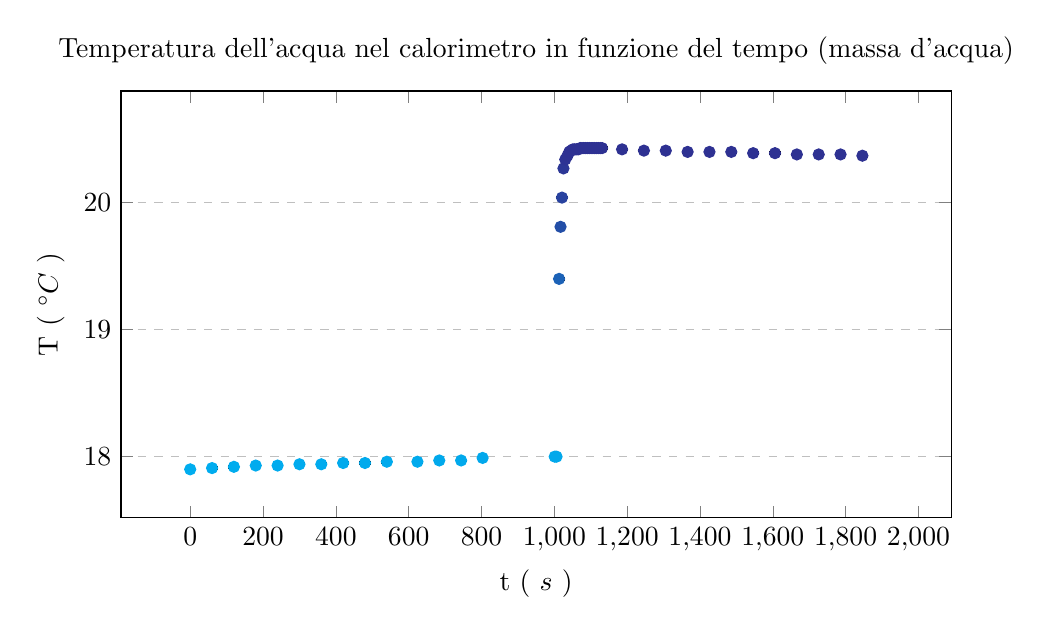
\begin{tikzpicture}
				\begin{axis}[
					title={Temperatura dell'acqua nel calorimetro in funzione del tempo (massa d'acqua)},
					xlabel={t ( $s$ )},
					ylabel={T ( $^\circ C$ )},
					xmin=0, xmax=1900,
					ymin=17.8, ymax=20.6,
					xtick={},
					ytick={},
					legend pos=north west,
					ymajorgrids=true,
					grid style=dashed,
					enlargelimits=0.1,
					width=\textwidth,
					height=7cm,
					point meta min=17.9,
					point meta max=20.4,
					colormap={yellowred}{
						color(0cm)=(cyan)
						color(1cm)=(blue)
					},
					]
					
					% Define the data
					\pgfplotstableread{
						x y yerr
						0.00 17.90 0.01
						60.00 17.91 0.01
						120.00 17.92 0.01
						180.00 17.93 0.01
						240.00 17.93 0.01
						300.00 17.94 0.01
						360.00 17.94 0.01
						420.00 17.95 0.01
						480.00 17.95 0.01
						540.00 17.96 0.01
						624.00 17.96 0.01
						684.00 17.97 0.01
						744.00 17.97 0.01
						803.00 17.99 0.01
						1001.00 18.00 0.01
						1006.00 18.00 0.01
						1013.00 19.4 0.01
						1017.00 19.81 0.01
						1021.00 20.04 0.01
						1025.00 20.27 0.01
						1030.00 20.34 0.01
						1036.00 20.37 0.01
						1041.00 20.40 0.01
						1046.00 20.41 0.01
						1051.00 20.42 0.01
						1056.00 20.42 0.01
						1061.00 20.42 0.01
						1066.00 20.42 0.01
						1071.00 20.43 0.01
						1076.00 20.43 0.01
						1081.00 20.43 0.01
						1086.00 20.43 0.01
						1091.00 20.43 0.01
						1096.00 20.43 0.01
						1101.00 20.43 0.01
						1106.00 20.43 0.01
						1111.00 20.43 0.01
						1116.00 20.43 0.01
						1121.00 20.43 0.01
						1126.00 20.43 0.01
						1131.00 20.43 0.01
						1186.00 20.42 0.01
						1246.00 20.41 0.01
						1306.00 20.41 0.01
						1366.00 20.40 0.01
						1426.00 20.40 0.01
						1486.00 20.40 0.01
						1546.00 20.39 0.01
						1606.00 20.39 0.01
						1666.00 20.38 0.01
						1726.00 20.38 0.01
						1786.00 20.38 0.01
						1846.00 20.37 0.01
						
					} \datatable
					
					% Plot the data with gradient
					\addplot[
					scatter, 
					only marks, 
					scatter src=explicit,
					scatter/use mapped color={
						draw=mapped color,
						fill=mapped color
					},
					error bars/.cd,
					y dir=both, y explicit
					]
					table[x=x, y=y, y error=yerr, meta=y] {\datatable};
				\end{axis}
			\end{tikzpicture}
		\end{figure}
	\end{center}
	
	Come per il cilindro metallico viene rilevata la temperatura dell'acqua nel calorimetro ogni minuto fino all'istante di versamento della massa d'acqua \(m'_{a}\) riscaldata nel bollitore. Dal versamento fino alla stabilizzazione della temperatura le misure sono effettuate a intervalli di 5 secondi e poi nuovamente di un minuto.
	
	\subsubsection{Fit lineare \(T'_{\text{eq}}\)}
	In questo caso è nota la temperatura \(T'_{1}\) corrispondente alla temperatura all'istante di versamento della massa d'acqua e vale \(T'_{1} = (18.00 \pm 0.01)^\circ C\).
	
	Invece per trovare \(T'_{\text{eq}}\) si procede al fit lineare  delle ultime misure.
	
	
	\begin{center}
		\begin{figure}[H]
			\centering
			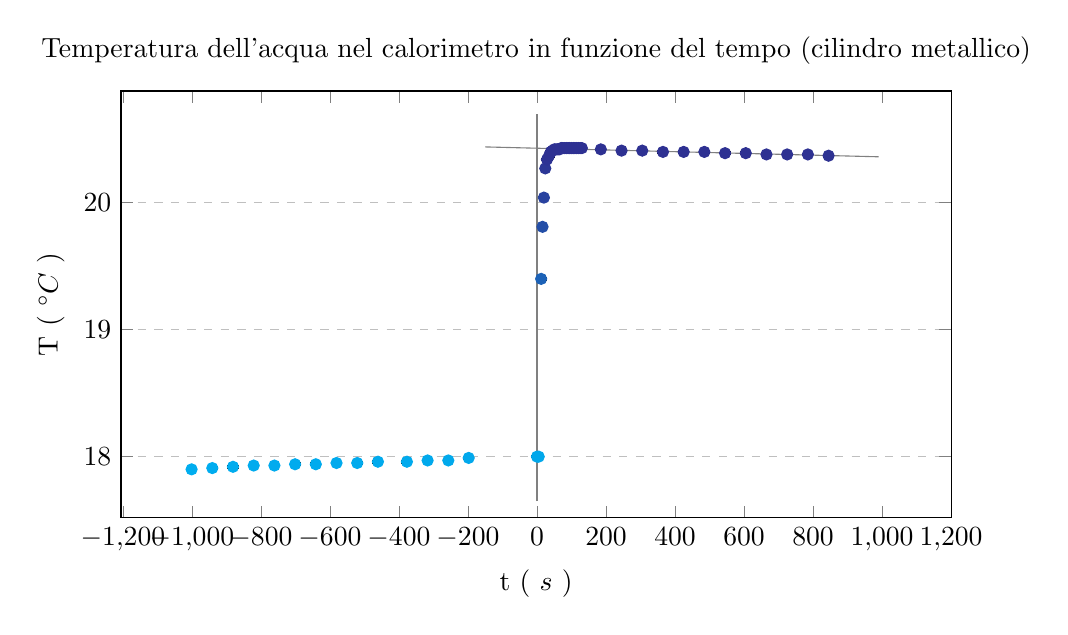
\begin{tikzpicture}
				\begin{axis}[
					title={Temperatura dell'acqua nel calorimetro in funzione del tempo (cilindro metallico)},
					xlabel={t ( $s$ )},
					ylabel={T ( $^\circ C$ )},
					xmin=-1005, xmax=1000,
					ymin=17.8, ymax=20.6,
					xtick={},
					ytick={},
					legend pos=north west,
					ymajorgrids=true,
					grid style=dashed,
					enlargelimits=0.1,
					width=\textwidth,
					height=7cm,
					point meta min=17.9,
					point meta max=20.4,
					colormap={yellowred}{
						color(0cm)=(cyan)
						color(1cm)=(blue)
					},
					]
					
					% Define the data
					\pgfplotstableread{
						x y yerr
						-1001 17.90 0.01
						-941 17.91 0.01
						-881 17.92 0.01
						-821 17.93 0.01
						-761 17.93 0.01
						-701 17.94 0.01
						-641 17.94 0.01
						-581 17.95 0.01
						-521 17.95 0.01
						-461 17.96 0.01
						-377 17.96 0.01
						-317 17.97 0.01
						-257 17.97 0.01
						-198 17.99 0.01
						0 18.00 0.01
						5 18.00 0.01
						12 19.4 0.01
						16 19.81 0.01
						20 20.04 0.01
						24 20.27 0.01
						29 20.34 0.01
						35 20.37 0.01
						40 20.40 0.01
						45 20.41 0.01
						50 20.42 0.01
						55 20.42 0.01
						60 20.42 0.01
						65 20.42 0.01
						70 20.43 0.01
						75 20.43 0.01
						80 20.43 0.01
						85 20.43 0.01
						90 20.43 0.01
						95 20.43 0.01
						100 20.43 0.01
						105 20.43 0.01
						110 20.43 0.01
						115 20.43 0.01
						120 20.43 0.01
						125 20.43 0.01
						130 20.43 0.01
						185 20.42 0.01
						245 20.41 0.01
						305 20.41 0.01
						365 20.40 0.01
						425 20.40 0.01
						485 20.40 0.01
						545 20.39 0.01
						605 20.39 0.01
						665 20.38 0.01
						725 20.38 0.01
						785 20.38 0.01
						845 20.37 0.01
						
					} \datatable
					
					% Plot the data with gradient
					\addplot[
					scatter, 
					only marks, 
					scatter src=explicit,
					scatter/use mapped color={
						draw=mapped color,
						fill=mapped color
					},
					error bars/.cd,
					y dir=both, y explicit
					]
					table[x=x, y=y, y error=yerr, meta=y] {\datatable};
					
					% Add vertical line at x=0
					\addplot [
					domain=15:18,
					samples=2,
					color=gray,
					]
					coordinates {(0,17.65) (0,20.7)};
					
					\addplot [
					domain=-150:990,
					samples=100,
					color=gray,
					]
					{20.429 - 0.000068181818181745*x};
				\end{axis}
			\end{tikzpicture}
		\end{figure}
	\end{center}
	
	\vspace{-1cm}
	\begin{minipage}{0.3\textwidth}
		\begin{table}[H]
			\centering
			\begin{tabular}{@{}cc@{}}
				\multicolumn{2}{c}{$\mathbf{T'_{\text{eq}}}$} \\ \midrule
				$\boldsymbol{t(s)}$ & $\boldsymbol{(T \pm 0.01) ^\circ C}$  \\ \midrule
				245	& 	$20.41$   \\\hdashline
				305	& 	$20.41$  \\\hdashline
				365	& 	$20.40$  \\\hdashline
				425	& 	$20.40$   \\\hdashline
				485	& 	$20.40$  \\\hdashline
				545	& 	$20.39$   \\\hdashline
				605	& 	$20.39$   \\\hdashline
				665	& 	$20.38$   \\\hdashline
				725	& 	$20.38$   \\\hdashline
				785	& 	$20.38$   \\ \hdashline
				845	& 	$20.37$  \\ \bottomrule   
			\end{tabular}
		\end{table}
	\end{minipage}
	\begin{minipage}{0.7\textwidth}
		Con il metodo dei minimi quadrati si trovano i parametri \(\boldsymbol{a}\) e \(\boldsymbol{b}\) della retta:
		\[ 
		y = \boldsymbol{a} + \boldsymbol{b} x
		\]
		\[ 
		\boldsymbol{a = 20.43 \pm 0.01} \qquad \qquad \boldsymbol{b = -0.00007 \pm 0.00001}
		\]
		
		
		Per verificare che la retta trovata si adatti bene ai dati è bene effettuare un test del \(\chi^2\).
	\end{minipage}
	
	\paragraph{Ipotesi nulla} La retta \(y = \boldsymbol{a} + \boldsymbol{b}x\) descrive bene l’andamento dei dati osservati sperimentalmente.
	
	
	\begin{table}[H] \centering
		%\ra{1.3}
		\begin{small}
			\begin{tabular}{@{}lcr@{}}\toprule
				\multicolumn{3}{c}{\textbf{valori per test} \(\boldsymbol{\chi^2}\)}\\ \midrule
				\textbf{Livello di significatività}		 &  \(\alpha\) &\(0.05\) \\  \hdashline
				\textbf{Gradi di libertà}		 & \(n\)  &\((11-2) = 9\) \\   \hdashline
				\textbf{Valore di} \(\boldsymbol{\chi^2}\)	 & \(\chi^2\)  &\(0.99\)\\  \hdashline
				\(\boldsymbol{\chi^2}\) \textbf{sospetto}		& \(\chi^2_{\text{sos}}\)  &\(3.32\)\\ \hdashline
				\(\boldsymbol{\chi^2}\) \textbf{critico}		& \(\chi^2_{\text{cri}}\)  &\(16.92\)\\ 
				\bottomrule
			\end{tabular}
		\end{small}
		\caption{\(\chi^2\) \(T'_{\text{eq}}\)}
	\end{table}
	
	\noindent
	Il valore \(\chi^2\) rilevato è sospetto, tuttavia, come per i fit precedenti, l'unica spiegazione che si può dare a tale risultato è una presa dati molto precisa; non si può pensare a barre d'errore troppo grandi poiché l'errore sulla temperatura è la sensibilità dello strumento. Accettando l'ipotesi nulla con un livello di significatività del 5\%.
	
	
	\begin{es}{\(T'_{1}\) e \(T'_{\text{eq}}\)}
		Conclusa l'analisi delle misure si ha \(T'_{1}\), di cui si ha la misura diretta, e \(T'_{\text{eq}}\)
		\[ 
		\azzurro{\boldsymbol{T'_{1} = 18.00 \pm 0.01}}\qquad \qquad \blu{\boldsymbol{T_{\text{eq}} = 20.43 \pm 0.01}}
		\]
	\end{es}
	
	
	\subsection{Calcolo massa equivalente e calore specifico}\label{calcolo me e cx}
	Dalle misure appena concluse è possibile trovare il valore della massa equivalente:
	\[ 
	m_{e} = \frac{m'_{a}\left(T'_{2} - T'_{\text{eq}}\right)}{T'_{\text{eq}} - T'_{1}} - m_{a(2)} \pm \sigma_{m_e} =  \frac{m'_{a}\Delta T'_{2e}}{\Delta T'_{e1}} - m_{a(2)}\pm \sigma_{m_e} \footnotemark\footnotetext{\label{errore in appendice}Lo sviluppo dell'errore di \(m_{e}\) e di \(c_{x}\) è riportato in appendice (\ref{sigma me})}
	\]

	\begin{table}[H] \centering
		%\ra{1.3}
		\begin{small}
			\begin{tabular}{@{}lcccr@{}}\toprule
								&  	\textbf{misure}	& \textbf{errore assoluto} & \textbf{errore relativo}  & u.m.\\ \midrule
				\(\Delta T'_{2e}\)	&  \(61.6\)	& \(0.1\)	& \(0.002\)	&\(^\circ C\)			\\  \hdashline
				\(\Delta T'_{e1}\)	&  \(2.43\)	& \(0.01\)	& \(0.01\)	&\(^\circ C\)			\\  \hdashline
				\(m'_{a}\)			&  \(0.1116\)	& \(0.0002\)	& \(0.002\)	&\(\SI{}{\kilogram}\) 	 \\  \hdashline
				\(m_{a(2)}\)		    &  \(2.6000\)    & \(0.0002\)	& \(0.0001\)	&\(\SI{}{\kilogram}\) 	\\ \bottomrule
			\end{tabular}
			\caption{misure per massa equivalente}
			\label{table:Tabella massa eqiuivalente 1}
		\end{small}
	\end{table}
	
	
	\[ 
	\boxed{\boldsymbol{m_{e} = (0.22 \pm 0.02)\SI{}{\kilogram}}}
	\]
	
	\noindent
	Ora si hanno tutti i dati per calcolare il calore specifico del corpo \(c_{x}\):
	
	\[ 
	c_{x} = \frac{(m_{e} + m_{a})c_{a}(T_{e} - T_{1})}{m_{c}(T_{2}-T_{e})} \pm \sigma_{c_x} = \frac{Mc_{a}}{m_{c}}\frac{\Delta T_{e1}}{\Delta T_{2e}}\pm \sigma_{c_x} 
	\]
	con \(c_{a} = 1 \frac{\text{cal}}{g ^\circ C}\)
	\begin{table}[H] \centering
		%\ra{1.3}
		\begin{small}
			\begin{tabular}{@{}lcccr@{}}\toprule
				&  	\textbf{misure}	& \textbf{errore assoluto} & \textbf{errore relativo}  & u.m.\\ \midrule
				\(\Delta T_{e1}\)	&  \(68\)	& \(1\)	& \(0.02\)	&\(^\circ C\)			\\  \hdashline
				\(\Delta T_{2e}\)	&  \(2.17\)	& \(0.03\)	& \(0.01\)	&\(^\circ C\)			\\  \hdashline
				\(M\)		    &  \(2.83\)    & \(0.02\)	& \(0.005\)	&\(\SI{}{\kilogram}\) 	\\  \bottomrule
			\end{tabular}
			\caption{misure per calore specifico}
			\label{table:Tabella calore specifico 1}
		\end{small}
	\end{table}
	
	\[ 
	\boxed{\boldsymbol{c_{x} = (0.233 \pm 0.005) \frac{\text{cal}}{g ^\circ C}}}
	\]
	
	\subsection{Analisi errori}
	Visti i risultati ottenuti è possibile ripetere l'esperienza modificando alcuni parametri iniziali così da ottenere un calore specifico e una massa equivalente più accurati. Per fare ciò si vanno a confrontare gli errori relativi dei fattori delle due espressioni e si individua quale di questi è il maggiore (e quindi è più responsabile dell'aumentare delle incertezze).
	
	Tra i fattori di \(m_{e}\) si nota subito che l'errore relativo di \(\Delta T'_{e1} = T'_{\text{eq}} - T'_{1}\) è di un ordine di grandezza superiore agli altri; invece tra i fattori di \(c_{x}\) sia \(\Delta T_{2e}=T_{2} - T_{\text{eq}}\) sia \(\Delta T_{e1} = T_{\text{eq}} - T_{1}\) risultano di un ordine di grandezza superiori agli altri. 
	
	Anche aumentare \(m_{a}\) massa d'acqua iniziale aiuterebbe anche se in miusra minore.
	
	Per far si che nella prossima presa dati questi errori relativi diminuiscano decidiamo di aumentare i delta in questo modo:
	\begin{enumerate}
		\item Diminuire la temperatura iniziale cominciando con \(T_{1}\) e \(T'_{1}\) minori;
		\item Aumentare la temperatura finale comnciando con la temperatura del corpo \(T_{2}\) maggiore;
		\item Aumentare la massa d'acqua nel calorimetro così che \(M\) risulti maggiore.
	\end{enumerate}
	
	
	
	
	\newpage
	\section{Seconda presa dati}
	\subsection{Cilindro metallico}
	
	\begin{minipage}{0.4\textwidth}
		\begin{table}[H] \centering
			%\ra{1.3}
			\begin{small}
				\begin{tabular}{@{}lrr@{}}\toprule
					\textbf{Oggetto}& &  \(\boldsymbol{(m \pm 0.0001) \SI{}{\kilogram}}\) \\ \midrule
					\textbf{Massa vaso}	&	 & \(1.3760\)   \\  \hdashline
					\textbf{Massa vaso + acqua}	&	 & \(4.1790\)   \\  \hdashline
					\textbf{Massa corpo}	& \(m_{c}\)	 & \(0.3866\)   \\  \hdashline
					\textbf{Massa becher}	&	 & \(0.2290\)   \\
					\bottomrule
				\end{tabular}
			\end{small}
			\caption{Misure preliminari (masse)}
		\end{table}
	\end{minipage}
	\begin{minipage}{0.6\textwidth}
		\begin{table}[H] \centering
			%\ra{1.3}
			\begin{small}
				\begin{tabular}{@{}lrr@{}}\toprule
					\textbf{Oggetto}					&  			& \textbf{(\(\boldsymbol{T}\))} \(\boldsymbol{^\circ C}\))\\ \midrule
					\textbf{Temp. cilindro metallico}	& 	\(T_{2}\)		& \(94 \pm 1\)	 \\  \hdashline
					\textbf{Temp. acqua}				&					&\(12.95 \pm 0.01\)		 	 \\  \hdashline
					\textbf{Temp. ambiente}				&					& \(19 \pm 1\)		 	  \\  
					\bottomrule
				\end{tabular}
			\end{small}
			\caption{Misure preliminari (temperature)}
		\end{table}
	\end{minipage}
	\vspace{1cm}
	
	Dalle seguenti misure si ricava la massa d'acqua \(m_{a}\) presente nel calorimetro come differenza della massa del vaso più l'acqua e la massa del vaso: \(\boldsymbol{(m_{a} = 2.8030\pm 0.0002)\SI{}{\kilogram}}\). \\
	
	\noindent
	Immerso il cilindro metallico nell'acqua del calorimetro si acquisisce la temperatura dell'acqua a intervalli di \(5 s\) fino a che questa non raggiuge una soglia di equilibrio. Una volta raggiunta la temperatura di equilibrio si acquisisce nuovamente a intervalli di un minuto.
	
		\begin{center}
		\begin{figure}[H]
			\centering
			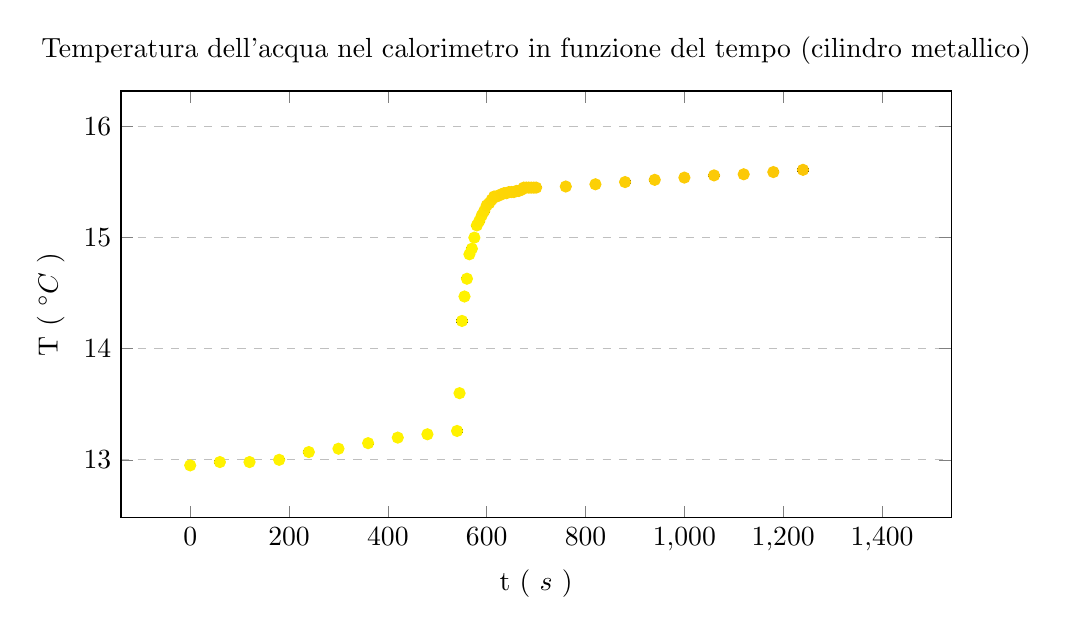
\begin{tikzpicture}
				\begin{axis}[
					title={Temperatura dell'acqua nel calorimetro in funzione del tempo (cilindro metallico)},
					xlabel={t ( $s$ )},
					ylabel={T ( $^\circ C$ )},
					xmin=0, xmax=1400,
					ymin=12.8, ymax=16,
					xtick={},
					ytick={},
					legend pos=south east,
					ymajorgrids=true,
					grid style=dashed,
					enlargelimits=0.1,
					width=\textwidth,
					height=7cm,
					point meta min=15,
					point meta max=18,
					colormap={yellowred}{
						color(0cm)=(yellow)
						color(1cm)=(red)
					},
					]
					
					% Define the data
					\pgfplotstableread{
						x y yerr
						0 12.95 0.01
						60 12.98 0.01
						120 12.98 0.01
						180 13 0.01
						240 13.07 0.01
						300 13.1 0.01
						360 13.15 0.01
						420 13.2 0.01
						480 13.23 0.01
						540 13.26 0.01
						545 13.6 0.01
						550 14.25 0.01
						555 14.47 0.01
						560 14.63 0.01
						565 14.85 0.01
						570 14.9 0.01
						575 15 0.01
						580 15.11 0.01
						585 15.15 0.01
						590 15.2 0.01
						595 15.24 0.01
						600 15.29 0.01
						605 15.31 0.01
						610 15.34 0.01
						615 15.37 0.01
						620 15.37 0.01
						625 15.38 0.01
						630 15.39 0.01
						635 15.4 0.01
						640 15.4 0.01
						645 15.41 0.01
						650 15.41 0.01
						655 15.41 0.01
						660 15.42 0.01
						665 15.42 0.01
						670 15.43 0.01
						675 15.45 0.01
						680 15.45 0.01
						685 15.45 0.01
						690 15.45 0.01
						695 15.45 0.01
						700 15.45 0.01
						760 15.46 0.01
						820 15.48 0.01
						880 15.5 0.01
						940 15.52 0.01
						1000 15.54 0.01
						1060 15.56 0.01
						1120 15.57 0.01
						1180 15.59 0.01
						1240 15.61 0.01
					} \datatable
					
					% Plot the data with gradient
					\addplot[
					scatter, 
					only marks, 
					scatter src=explicit,
					scatter/use mapped color={
						draw=mapped color,
						fill=mapped color
					},
					error bars/.cd,
					y dir=both, y explicit
					]
					table[x=x, y=y, y error=yerr, meta=y] {\datatable};
				\end{axis}
			\end{tikzpicture}
		\end{figure}
	\end{center}
	
	
	\subsubsection{Fit lineare \(T_{\text{eq}}\)}
	La temperatura iniziale \(T_{1}\) è quella corrispondente all'istante di immersione del corpo e vale \(T_{1} = (	13.26 \pm 0.01)^\circ C\)
	
	
	Per ricavare \(T_{\text{eq}}\) si trasla il grafico portando l'istante di immersione sullo zero e si traccia  la retta di best fit delle temperature finali.
	\noindent
	Per prima cosa troviamo \(T_{\text{eq}}\):
		\begin{center}
		\begin{figure}[H]
			\centering
			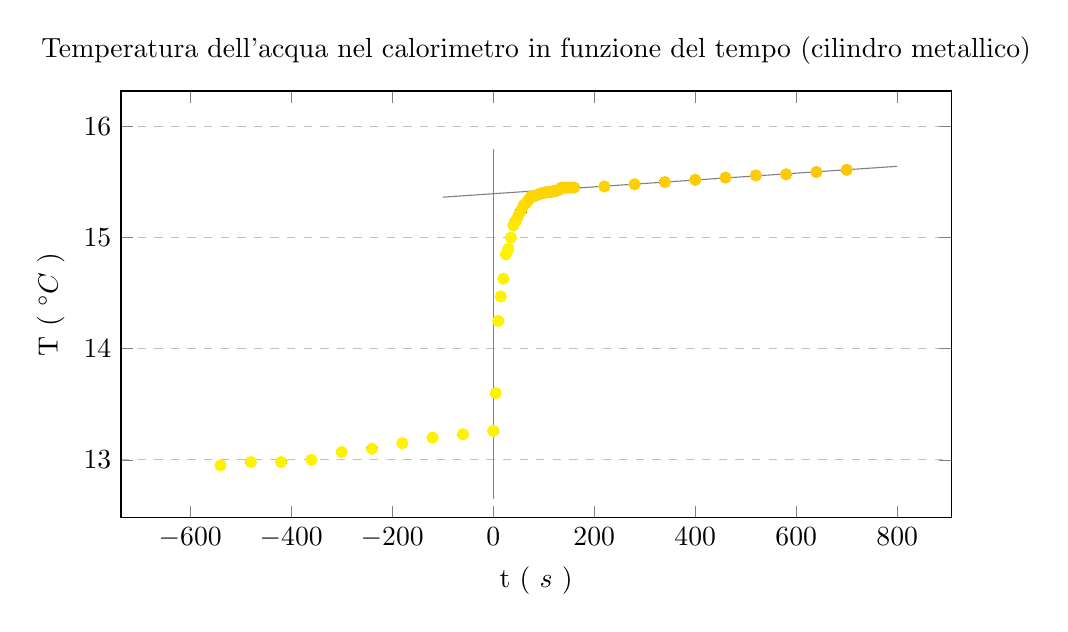
\begin{tikzpicture}
				\begin{axis}[
					title={Temperatura dell'acqua nel calorimetro in funzione del tempo (cilindro metallico)},
					xlabel={t ( $s$ )},
					ylabel={T ( $^\circ C$ )},
					xmin=-600, xmax=770,
					ymin=12.8, ymax=16,
					xtick={},
					ytick={},
					legend pos=south east,
					ymajorgrids=true,
					grid style=dashed,
					enlargelimits=0.1,
					width=\textwidth,
					height=7cm,
					point meta min=15,
					point meta max=18,
					colormap={yellowred}{
						color(0cm)=(yellow)
						color(1cm)=(red)
					},
					]
					
					% Define the data
					\pgfplotstableread{
						x y yerr
						-540 12.95 0.01
						-480 12.98 0.01
						-420 12.98 0.01
						-360 13 0.01
						-300 13.07 0.01
						-240 13.1 0.01
						-180 13.15 0.01
						-120 13.2 0.01
						-60 13.23 0.01
						0 13.26 0.01
						5 13.6 0.01
						10 14.25 0.01
						15 14.47 0.01
						20 14.63 0.01
						25 14.85 0.01
						30 14.9 0.01
						35 15 0.01
						40 15.11 0.01
						45 15.15 0.01
						50 15.2 0.01
						55 15.24 0.01
						60 15.29 0.01
						65 15.31 0.01
						70 15.34 0.01
						75 15.37 0.01
						80 15.37 0.01
						85 15.38 0.01
						90 15.39 0.01
						95 15.4 0.01
						100 15.4 0.01
						105 15.41 0.01
						110 15.41 0.01
						115 15.41 0.01
						120 15.42 0.01
						125 15.42 0.01
						130 15.43 0.01
						135 15.45 0.01
						140 15.45 0.01
						145 15.45 0.01
						150 15.45 0.01
						155 15.45 0.01
						160 15.45 0.01
						220 15.46 0.01
						280 15.48 0.01
						340 15.5 0.01
						400 15.52 0.01
						460 15.54 0.01
						520 15.56 0.01
						580 15.57 0.01
						640 15.59 0.01
						700 15.61 0.01
					} \datatable
					
					% Plot the data with gradient
					\addplot[
					scatter, 
					only marks, 
					scatter src=explicit,
					scatter/use mapped color={
						draw=mapped color,
						fill=mapped color
					},
					error bars/.cd,
					y dir=both, y explicit
					]
					table[x=x, y=y, y error=yerr, meta=y] {\datatable};
					% Add vertical line at x=0
					\addplot [
					domain=15:18,
					samples=2,
					color=gray,
					]
					coordinates {(0,12.65) (0,15.8)};
					
					\addplot [
					domain=-100:800,
					samples=100,
					color=gray,
					]
					{15.395 + 0.000308333333333299*x};
				\end{axis}
			\end{tikzpicture}
		\end{figure}
	\end{center}
	\vspace{-1cm}
	\begin{minipage}{0.3\textwidth}
		\begin{table}[H]
			\centering
			\begin{tabular}{@{}cc@{}}
				\multicolumn{2}{c}{$\mathbf{T_{\text{eq}}}$} \\ \midrule
				$\boldsymbol{t(s)}$ & $\boldsymbol{(T \pm 0.01) ^\circ C}$  \\ \midrule
				220 & 15.46 \\ \hdashline
				280 & 15.48 \\ \hdashline
				340 & 15.50 \\ \hdashline
				400 & 15.52 \\ \hdashline
				460 & 15.54 \\ \hdashline
				520 & 15.56 \\ \hdashline
				580 & 15.57 \\ \hdashline
				640 & 15.59 \\ \hdashline
				700 & 15.60 \\ \bottomrule
			\end{tabular}
		\end{table}
	\end{minipage}
	\begin{minipage}{0.7\textwidth}
		 Con il metodo dei minimi quadrati si trovano i parametri \(\boldsymbol{a}\) e \(\boldsymbol{b}\) della retta:
		\[ 
		y = \boldsymbol{a} + \boldsymbol{b} x
		\]
		\[ 
		\boldsymbol{a = 15.40	 \pm 0.01} \qquad \qquad \boldsymbol{b = 0.00031 \pm 0.00002}
		\]
		
		
		Per verificare che la retta trovata si adatti bene ai dati è bene effettuare un test del \(\chi^2\).
	\end{minipage}
	
	\paragraph{Ipotesi nulla} La retta \(y = \boldsymbol{a} + \boldsymbol{b}x\) descrive bene l’andamento dei dati osservati sperimentalmente.
	
	
	\begin{table}[H] \centering
		%\ra{1.3}
		\begin{small}
			\begin{tabular}{@{}lcr@{}}\toprule
				\multicolumn{3}{c}{\textbf{valori per test} \(\boldsymbol{\chi^2}\)}\\ \midrule
				\textbf{Livello di significatività}		 &  \(\alpha\) &\(0.05\)\footnotemark \\  \hdashline
				\textbf{Gradi di libertà}		 & \(n\)  &\((9-2) = 7\) \\   \hdashline
				\textbf{Valore di} \(\boldsymbol{\chi^2}\)	 & \(\chi^2\)  &\(0.65\)\\  \hdashline
				\(\boldsymbol{\chi^2}\) \textbf{sospetto}		& \(\chi^2_{\text{sos}}\)  &\(2.17\)\\ \hdashline
				\(\boldsymbol{\chi^2}\) \textbf{critico}		& \(\chi^2_{\text{cri}}\)  &\(114.07\)\\ 
				\bottomrule
			\end{tabular}
		\end{small}
		\caption{\(\chi^2\) \(T_{1}\)}
	\end{table}
	
	\noindent
	Il valore \(\chi^2\) rilevato è minore di quello sospetto: un piccolo valore di \(\chi^2\) è indice di barre d'errore troppo grandi o di una forte vicinanza tra valori sperimentali e valori teorici. A corroborare l'ipotesi di una presa dati molto precisa si rileva un coefficiente di correlazione lineare \(r = 0.997\). Inoltre l'errore associato alla temperatura (\(0.01 ^\circ C\)) è la sensibilità del termometro utilizzato e quindi non può essere stato sovrastimato. Concludo quindi accettando l'ipotesi nulla con un livello di significatività del 5\%.
	
	\begin{es}{\(T_{1}\) e \(T_{\text{eq}}\)}
		\[ 
		\giallo{\boldsymbol{T_{1} = 13.26	\pm 0.01}}\qquad \qquad \rosso{\boldsymbol{T_{\text{eq}} = 15.50	\pm 0.01}}
		\]
	\end{es}
	
	\subsection{Massa d'acqua}
	\begin{minipage}{0.4\textwidth}
		\begin{table}[H] \centering
			%\ra{1.3}
			\begin{small}
				\begin{tabular}{@{}lrr@{}}\toprule
					\textbf{Oggetto}&  & \(\boldsymbol{(m \pm 0.0001) \SI{}{\kilogram}}\) \\ \midrule
					\textbf{Massa becher}	&	 & \(0.1046\)   \\  \hdashline
					\textbf{Massa becher + corpo}	& 	 & \(0.4939\)   \\  \hdashline
					\textbf{Massa corpo}	& \(m_{c}\)	 & \(0.3866\)   \\  \hdashline
					\textbf{Massa borraccia}	&	 & \(0.2544\)   \\\hdashline
					\textbf{Massa borraccia + acqua}	&	 & \(0.4047\)   \\  
					\bottomrule
				\end{tabular}
			\end{small}
			\caption{Misure preliminari (masse)}
		\end{table}
	\end{minipage}
	\begin{minipage}{0.6\textwidth}
		\begin{table}[H] \centering
			%\ra{1.3}
			\begin{small}
				\begin{tabular}{@{}lrr@{}}\toprule
					\textbf{Oggetto}					&  			& \textbf{(\(\boldsymbol{T}\)} \(\boldsymbol{^\circ C}\))\\ \midrule
					\textbf{Temp. acqua nella borraccia}	& 	\(T'_{2}\)		& \(82 \pm 0.1\)	 \\  \hdashline
					\textbf{Temp. acqua}				&					&\(17.90 \pm 0.01\)		 	 \\  \hdashline
					\textbf{Temp. ambiente}				&					& \(19 \pm 1\)		 	  \\  
					\bottomrule
				\end{tabular}
			\end{small}
			\caption{Misure preliminari (temperature)}
		\end{table}
	\end{minipage} \\
	\vspace{0.5cm}
	
	Nel momento dell'estrazione del corpo dal calorimetro parte dell'acqua in quest'utlimo potrebbe essere rimasta attaccata al corpo. Per ricavare la massa d'acqua rimasta nel calorimetro pesiamo la massa del corpo bagnato in un becher; si ricava la massa d'acqua \(m_{a(2)}\) presente nel calorimetro come:
	\begin{align*}
		\boldsymbol{	m_{a(2)} =}& m_{a} - (m_{\text{bercher+corpo}} - m_{\text{bercher}} - m_{\text{c}}) \\
		\boldsymbol{=}& \boldsymbol{(2.8010 \pm 0.0002) \SI{}{\kilogram}}
	\end{align*}
	Si ricava invece la massa d'acqua da versare togliendo la tara utilizzata (borraccia) alla massa borraccia più acqua:
	\[ 
	\boldsymbol{m'_{a} = (0.1503 \pm	0.0002)\SI{}{\kilogram}}
	\]
	Come per il cilindro metallico viene rilevata la temperatura dell'acqua nel calorimetro ogni minuto fino all'istante di versamento della massa d'acqua \(m'_{a}\) riscaldata nel bollitore. Dal versamento fino alla stabilizzazione della temperatura le misure sono effettuate a intervalli di 5 secondi e poi nuovamente di un minuto.
	
	\begin{center}
		\begin{figure}[H]
			\centering
			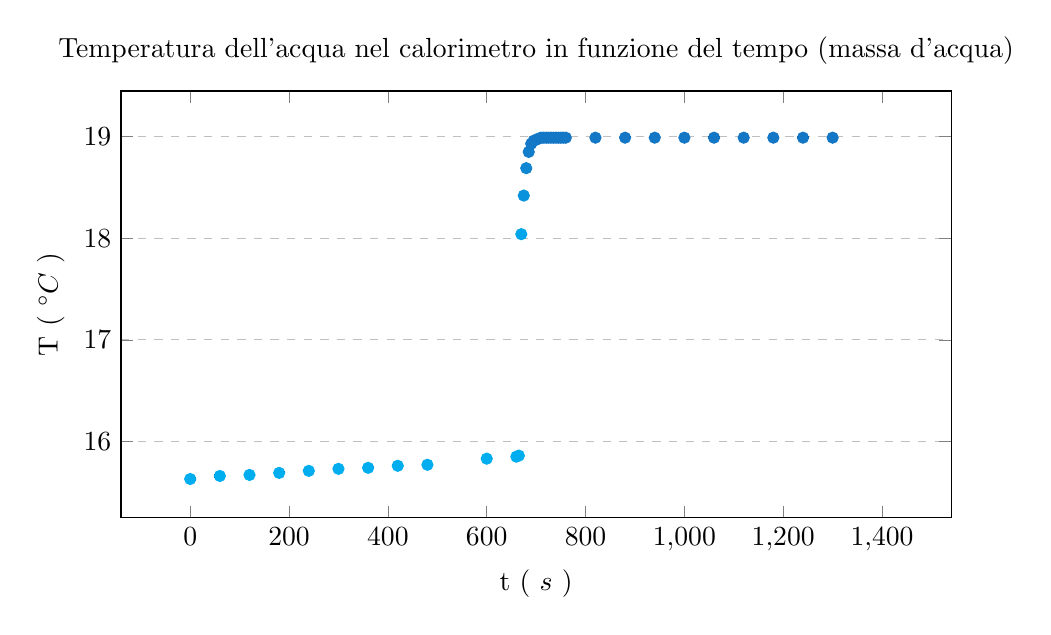
\begin{tikzpicture}
				\begin{axis}[
					title={Temperatura dell'acqua nel calorimetro in funzione del tempo (massa d'acqua)},
					xlabel={t ( $s$ )},
					ylabel={T ( $^\circ C$ )},
					xmin=0, xmax=1400,
					ymin=15.6, ymax=19.1,
					xtick={},
					ytick={},
					legend pos=north west,
					ymajorgrids=true,
					grid style=dashed,
					enlargelimits=0.1,
					width=\textwidth,
					height=7cm,
					point meta min=17.9,
					point meta max=20.4,
					colormap={yellowred}{
						color(0cm)=(cyan)
						color(1cm)=(blue)
					},
					]
					
					% Define the data
					\pgfplotstableread{
						x y yerr
						0 15.63 0.01
						60 15.66 0.01
						120 15.67 0.01
						180 15.69 0.01
						240 15.71 0.01
						300 15.73 0.01
						360 15.74 0.01
						420 15.76 0.01
						480 15.77 0.01
						600 15.83 0.01
						660 15.85 0.01
						665 15.86 0.01
						670 18.04 0.01
						675 18.42 0.01
						680 18.69 0.01
						685 18.85 0.01
						690 18.93 0.01
						695 18.96 0.01
						700 18.97 0.01
						705 18.98 0.01
						710 18.99 0.01
						715 18.99 0.01
						720 18.99 0.01
						725 18.99 0.01
						730 18.99 0.01
						735 18.99 0.01
						740 18.99 0.01
						745 18.99 0.01
						750 18.99 0.01
						755 18.99 0.01
						760 18.99 0.01
						820 18.99 0.01
						880 18.99 0.01
						940 18.99 0.01
						1000 18.99 0.01
						1060 18.99 0.01
						1120 18.99 0.01
						1180 18.99 0.01
						1240 18.99 0.01
						1300 18.99 0.01
					} \datatable
					
					% Plot the data with gradient
					\addplot[
					scatter, 
					only marks, 
					scatter src=explicit,
					scatter/use mapped color={
						draw=mapped color,
						fill=mapped color
					},
					error bars/.cd,
					y dir=both, y explicit
					]
					table[x=x, y=y, y error=yerr, meta=y] {\datatable};
					
				\end{axis}
			\end{tikzpicture}
		\end{figure}
	\end{center}
	
	\subsubsection{Fit lineare \(T'_{\text{eq}}\)}
	In questo caso è nota la temperatura \(T'_{1}\) corrispondente alla temperatura all'istante di versamento della massa d'acqua e vale \(T'_{1} = (15.85 \pm 0.01)^\circ C\).
	
	Invece per trovare \(T'_{\text{eq}}\) si procede al fit lineare  delle ultime misure.
	
	
	\begin{center}
		\begin{figure}[H]
			\centering
			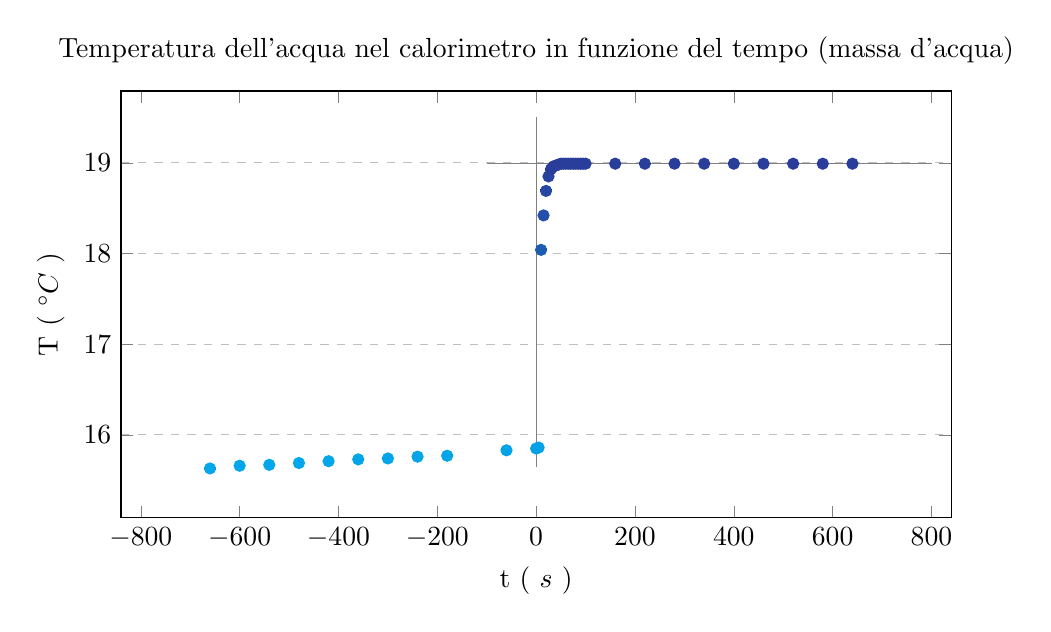
\begin{tikzpicture}
				\begin{axis}[
					title={Temperatura dell'acqua nel calorimetro in funzione del tempo (massa d'acqua)},
					xlabel={t ( $s$ )},
					ylabel={T ( $^\circ C$ )},
					xmin=-700, xmax=700,
					ymin=15.48, ymax=19.4,
					xtick={},
					ytick={},
					legend pos=north west,
					ymajorgrids=true,
					grid style=dashed,
					enlargelimits=0.1,
					width=\textwidth,
					height=7cm,
					point meta min=15.48,
					point meta max=19.4,
					colormap={yellowred}{
						color(0cm)=(cyan)
						color(1cm)=(blue)
					},
					]
					
					% Define the data
					\pgfplotstableread{
						x y yerr
						-660 15.63 0.01
						-600 15.66 0.01
						-540 15.67 0.01
						-480 15.69 0.01
						-420 15.71 0.01
						-360 15.73 0.01
						-300 15.74 0.01
						-240 15.76 0.01
						-180 15.77 0.01
						-60 15.83 0.01
						0 15.85 0.01
						5 15.86 0.01
						10 18.04 0.01
						15 18.42 0.01
						20 18.69 0.01
						25 18.85 0.01
						30 18.93 0.01
						35 18.96 0.01
						40 18.97 0.01
						45 18.98 0.01
						50 18.99 0.01
						55 18.99 0.01
						60 18.99 0.01
						65 18.99 0.01
						70 18.99 0.01
						75 18.99 0.01
						80 18.99 0.01
						85 18.99 0.01
						90 18.99 0.01
						95 18.99 0.01
						100 18.99 0.01
						160 18.99 0.01
						220 18.99 0.01
						280 18.99 0.01
						340 18.99 0.01
						400 18.99 0.01
						460 18.99 0.01
						520 18.99 0.01
						580 18.99 0.01
						640 18.99 0.01
					}  \datatable
					
					% Plot the data with gradient
					\addplot[
					scatter, 
					only marks, 
					scatter src=explicit,
					scatter/use mapped color={
						draw=mapped color,
						fill=mapped color
					},
					error bars/.cd,
					y dir=both, y explicit
					]
					table[x=x, y=y, y error=yerr, meta=y] {\datatable};
					% Add vertical line at x=0
					\addplot [
					domain=15:18,
					samples=2,
					color=gray,
					]
					coordinates {(0,15.65) (0,19.5)};
					
					\addplot [
					domain=-100:800,
					samples=100,
					color=gray,
					]
					{18.99};
				\end{axis}
			\end{tikzpicture}
		\end{figure}
	\end{center}
	
	\vspace{-1cm}
	\begin{minipage}{0.3\textwidth}
		\begin{table}[H]
			\centering
			\begin{tabular}{@{}cc@{}}
				\multicolumn{2}{c}{$\mathbf{T'_{\text{eq}}}$} \\ \midrule
				$\boldsymbol{t(s)}$ & $\boldsymbol{(T \pm 0.01) ^\circ C}$  \\ \midrule
				160 & 18.99 \\ \hdashline
				220 & 18.99 \\ \hdashline
				280 & 18.99 \\ \hdashline
				340 & 18.99 \\ \hdashline
				400 & 18.99 \\ \hdashline
				460 & 18.99 \\ \hdashline
				520 & 18.99 \\ \hdashline
				580 & 18.99 \\ \hdashline
				640 & 18.99 \\\bottomrule
			\end{tabular}
		\end{table}
	\end{minipage}
	\begin{minipage}{0.7\textwidth}
		Come si può notare le ultime misure sono tutte stabilizzate sulla temperatura ambiente (precedentemente misurata \((19 \pm 1) ^\circ C\)). Procedere al fit dei dati sarebbe inutile in quanto la retta in questione è
		\[ 
		y = (18.99 \pm 0.01)^\circ C
		\]
		Sappiamo quindi che il valore di \(T'_{\text{eq}}\) è \(T_{\text{eq}} = (18.99 \pm 0.01)^\circ C\)
	\end{minipage}
	
	
	\begin{es}{\(T'_{1}\) e \(T'_{\text{eq}}\)}
		Conclusa l'analisi delle misure si hanno
		\[ 
		\azzurro{\boldsymbol{T'_{1} = 15.85 \pm 0.01}}\qquad \qquad \blu{\boldsymbol{T_{\text{eq}} = 18.99 \pm 0.01}}
		\]
	\end{es}
	
	
	\subsection{Calcolo massa equivalente e calore specifico}\label{calcolo me e cx 2}
	Dalle misure appena concluse è possibile trovare il valore della massa equivalente:
	\[ 
	m'_{e} = \frac{m'_{a}\left(T'_{2} - T'_{\text{eq}}\right)}{T'_{\text{eq}} - T'_{1}} - m_{a(2)} \pm \sigma_{m'_e} =  \frac{m'_{a}\Delta T'_{2e}}{\Delta T'_{e1}} - m_{a(2)}\pm \sigma_{m'_e} \footnotemark\footnotetext{\label{errore in appendice}Lo sviluppo dell'errore di \(m_{e}\) e di \(c_{x}\) è riportato in appendice (\ref{sigma me})}
	\]
	
	\begin{table}[H] \centering
		%\ra{1.3}
		\begin{small}
			\begin{tabular}{@{}lcccr@{}}\toprule
				&  	\textbf{misure}	& \textbf{errore assoluto} & \textbf{errore relativo}  & u.m.\\ \midrule
				\(\Delta T'_{2e}\)	&  \(61.8\)	& \(0.1\)	& \(0.002\)	&\(^\circ C\)			\\  \hdashline
				\(\Delta T'_{e1}\)	&  \(3.14\)	& \(0.02\)	& \(0.005\)	&\(^\circ C\)			\\  \hdashline
				\(m'_{a}\)			&  \(0.1503\)	& \(0.0002\)	& \(0.001\)	&\(\SI{}{\kilogram}\) 	 \\  \hdashline
				\(m_{a(2)}\)		    &  \(2.8010\)    & \(0.0002\)	& \(0.0001\)	&\(\SI{}{\kilogram}\) 	\\ \bottomrule
			\end{tabular}
			\caption{misure per massa equivalente}
			\label{table:Tabella massa eqiuivalente 2}
		\end{small}
	\end{table}
	
	
	\[ 
	\boxed{\boldsymbol{m'_{e} = (0.206 \pm 0.001)\SI{}{\kilogram}}}
	\]
	
	\noindent
	Ora si hanno tutti i dati per calcolare il calore specifico del corpo \(c_{x}\):
	
	\[ 
	c'_{x} = \frac{(m'_{e} + m_{a})c_{a}(T_{e} - T_{1})}{m_{c}(T_{2}-T_{e})} \pm \sigma_{c_x} = \frac{Mc_{a}}{m_{c}}\frac{\Delta T_{e1}}{\Delta T_{2e}}\pm \sigma_{c_x} 
	\]
	con \(c_{a} = 1 \frac{\text{cal}}{g ^\circ C}\)
	\begin{table}[H] \centering
		%\ra{1.3}
		\begin{small}
			\begin{tabular}{@{}lcccr@{}}\toprule
				&  	\textbf{misure}	& \textbf{errore assoluto} & \textbf{errore relativo}  & u.m.\\ \midrule
				\(\Delta T_{e1}\)	&  \(2.14\)	& \(0.02\)	& \(0.007\)	&\(^\circ C\)			\\  \hdashline
				\(\Delta T_{2e}\)	&  \(78.6\)	& \(0.1\)	& \(0.001\)	&\(^\circ C\)			\\  \hdashline
				\(M\)		    &  \(3.006\)    & \(0.001\)	& \(0.0003\)	&\(\SI{}{\kilogram}\) 	\\  \bottomrule
			\end{tabular}
			\caption{misure per calore specifico}
			\label{table:Tabella calore specifico 2}
		\end{small}
	\end{table}
	
	\[ 
	\boxed{\boldsymbol{c'_{x} = (0.211 \pm 0.002) \frac{\text{cal}}{g ^\circ C}}}
	\]
	
	\newpage
	\section{Confronto masse equivalenti e calori specifici}
	Conclusa la seconda presa dati e ottenuti i valori del calore specifico del corpo e della massa equivalente del calorimetro si procede nella verifica che i risultati ottenuti nelle due prese dati siano compatibili tra di loro per scongiurare eventuali errori di procedura.
	
	\begin{table}[H] \centering
		%\ra{1.3}
		\begin{small}
			\begin{tabular}{@{}lccc@{}}
				&  	\textbf{misura}	& \textbf{errore assoluto} & \textbf{errore relativo}   \\ \bottomrule
				\(m_{e}\) & 0.22   & 0.02 & 9.1 \% \\ \hdashline
				\(m'_{e}\) &0.206 & 0.001 & 0.5 \% \\ \midrule
				\(c_{x}\) & 0.233 & 0.005& 2.1\%\\ \hdashline
				\(c'_{x}\) &0.211 & 0.002& 0.9 \%\\ \bottomrule
			\end{tabular}
			\caption{confronto prima e dopo correzion}
		\end{small}
	\end{table}
	
Si evince che le correzioni hanno permesso una stima di massa equivalente e calore specifico molto più precisa; tuttavia potrebbero risultare non compatibili i valori. Per accertarsi che i risultati della prima presa dati siano consistenti con quelli della seconda si sottopongono questi ultimi a un test \(z\). Più precisamente si va a verificare che la differenza tra \(c_{x}\) e \(c'_{x}\) e tra \(m_{e}\) e \(m'_{e}\) sia compatibile con \(0\):
\[ 
z = \frac{|m_e-m'_e|}{\sqrt{\sigma_{m_e}^2 + \sigma_{m'_e}^2}}  \qquad \qquad \qquad z = \frac{|c_{x}-c'_{x}|}{\sqrt{\sigma_{c_{x}}^2 + \sigma_{c'_{x}}^2}}
\]


\vspace{0.4cm}
\begin{center}
	\begin{minipage}{0.48\textwidth}
		\subsection{Test Z (\(m_{e}\))}
		\paragraph{Ipotesi nulla} I valori \(c_{x}\) e \(c'_{x}\) sono compatibili con un livello di signifatività del 5\%
		\begin{table}[H] \centering
			%\ra{1.3}
			\begin{small}
				\begin{tabular}{@{}lcr@{}}\toprule
					\multicolumn{3}{c}{\textbf{valori per test} \(\boldsymbol{z}\)}\\ \midrule
					\textbf{Livello di significatività}		 &  \(\alpha\) &\(0.05\) \\  \hdashline
					\(\boldsymbol{z}\) \textbf{osservato}		& \(z_{\text{oss}}\)  &\(0.7\)\\ \hdashline
					\(\boldsymbol{z}\) \textbf{critico}		& \(z_{\text{cri}}\)  &\(1.96\)\\ 
					\bottomrule
				\end{tabular}
			\end{small}
			\caption{\(z\) \(m_{e} - m'_{e}\)}
		\end{table}
	\end{minipage}
	\hspace{0.3cm}
	\begin{minipage}{0.48\textwidth}
		\subsection{Test Z (\(c_{x}\))}
		\paragraph{Ipotesi nulla}  I valori \(m_{e}\) e \(m'_{e}\) sono compatibili con un livello di signifatività del 5\%
		\begin{table}[H] \centering
			%\ra{1.3}
			\begin{small}
				\begin{tabular}{@{}lcr@{}}\toprule
					\multicolumn{3}{c}{\textbf{valori per test} \(\boldsymbol{z}\)}\\ \midrule
					\textbf{Livello di significatività}		 &  \(\alpha\) &\(0.05\) \\  \hdashline
					\(\boldsymbol{z}\) \textbf{osservato}		& \(z_{\text{oss}}\)  &\(4.0\)\\ \hdashline
					\(\boldsymbol{z}\) \textbf{critico}		& \(z_{\text{cri}}\)  &\(1.96\)\\ 
					\bottomrule
				\end{tabular}
			\end{small}
			\caption{\(z\) \(c_{x} - c'_{x}\)}
		\end{table}
	\end{minipage}
\end{center}

	Accetto la prima ipotesi nulla e rifiuto la seconda: le masse equivalenti risultano essere compatibili (livello di significatività del 5\%) mentre i calori speifici non lo sono. Una spiegazione plausibile è una prima presa dati imprecisa e più grossolana rispetto alla seconda che ha fornito un valore di \(c_{x}\) con errore di 0.9\% contro il 2.1\% della prima. Per accertarsi di quale calore specifico sia il più accurato li si confronta con il calore specifico dell'acciaio fornitoci dalla letteratura:
	\[ 
	c_{x_{\text{lett}}} = 0.215 \frac{\text{cal}}{g ^\circ C}
	\]
	
	\subsection{Test Z con calore specifico teorico}
	\paragraph{Iptesi nulla} Il calore specifico sperimentale (prima \(c_{x}\) e poi \(c'_{x}\)) è compatibile con il calore specifico fornito dalla letteratura
	
	\begin{center}
		\begin{minipage}{0.48\textwidth}
			\begin{table}[H] \centering
				%\ra{1.3}
				\begin{small}
					\begin{tabular}{@{}lcr@{}}\toprule
						\multicolumn{3}{c}{\textbf{valori per test} \(\boldsymbol{z}\)}\\ \midrule
						\textbf{Livello di significatività}		 &  \(\alpha\) &\(0.05\) \\  \hdashline
						\(\boldsymbol{z}\) \textbf{osservato}		& \(z_{\text{oss}}\)  &\(1.82\)\\ \hdashline
						\(\boldsymbol{z}\) \textbf{critico}		& \(z_{\text{cri}}\)  &\(1.96\)\\ 
						\bottomrule
					\end{tabular}
				\end{small}
				\caption{\(z\) \(c_{x} - c_{x_{\text{lett}}}\)}
			\end{table}
		\end{minipage}
		\hspace{0.3cm}
		\begin{minipage}{0.48\textwidth}
			\begin{table}[H] \centering
				%\ra{1.3}
				\begin{small}
					\begin{tabular}{@{}lcr@{}}\toprule
						\multicolumn{3}{c}{\textbf{valori per test} \(\boldsymbol{z}\)}\\ \midrule
						\textbf{Livello di significatività}		 &  \(\alpha\) &\(0.05\) \\  \hdashline
						\(\boldsymbol{z}\) \textbf{osservato}		& \(z_{\text{oss}}\)  &\(3.8\)\\ \hdashline
						\(\boldsymbol{z}\) \textbf{critico}		& \(z_{\text{cri}}\)  &\(1.96\)\\ 
						\bottomrule
					\end{tabular}
				\end{small}
				\caption{\(z\) \(c'_{x} - c_{x_{\text{lett}}}\)}
			\end{table}
		\end{minipage}
	\end{center}
	
	Come ci si poteva aspettare il primo calore specifico non risulta compatibile con quello teorico, mentre il secondo, frutto della presa dati più precisa, risulta compatibile (con un livello di significatività del 5\%). L'esito positivo del secondo test \(z\) evidenzia, oltre alla già verificata precisione, l'accuratezza dei valori ottenuti nella seconda procedura (rispetto alla prima). 
	
 

	
	
	\section{Errori sistematici}
	Per accertarsi che nessun fattore esterno abbia influenzato in modo significativo le prese dati si studiano i contributi energetici dell'agitatore e dell'ambiente esterno nel quale viene dispersa parte del calore.
	
	\subsection{Influenza agitatore}
	
	
	Il motorino elettrico che muove l'agitatore eroga una potenza di \(\SI{3}{\watt}\). Se si ipotizzasse per assurdo che tutta l’energia elettrica venisse convertita in calore, l'aumento di temperatura causato dal movimento dell’agitatore in un intervallo di tempo sarebbe:
	\[ 
	P = \frac{Q_{\text{ass}}}{\Delta t} = \frac{(m_{a} + m_{e})c_{a}\Delta T}{\Delta t} \quad \to \quad \Delta T = \frac{P\Delta t}{(m_{a} + m_{e})c_{a}}
	\]
	In un intervallo di tempo pari a circa \(1800\) secondi si ha una variazione di temperatura pari a 
	\[ 
	\Delta T = 0.45 ^\circ C 
	\]
	pari a crica 
	\[
	0.007 \frac{^\circ C}{60 s}
	\]
	Una variazione di \(0.007 ^\circ C\) al minuto non è apprezzabile dal termometro utilizzato nel calorimetro (sensibilità \(0.01^\circ C\))
	\subsection{Calore disperso}
	
	\newpage
	\section{Appendice}
	\subsection{Calcoli e approssimazioni ricorrenti}
	\begin{enumerate}
		\item L'errore di misure derivate da somme e differenze sono tutti ricavati come semplici somme in quadratura.
		\item Se l'errore associato a una misura derivata da una somma o una differenza era del tipo \(0.14\), \(0.014\), \(0.00\dots 014\) è sempre stato approssimato per eccesso. Si è preferito avere errori lievemente maggiori ma più realistici.
	\end{enumerate}
	
	\subsection{Calcolo \(T_{1}\) e \(T_{\text{eq}}\) con covarianze} \label{covarianza}
	Al fine di semplificare la ricerca di temperatura iniziale e temperatura di equilibrio è utile traslare i grafici portando l'istante d'immersione (prima del corpo poi della massa d'acqua) sullo \(0\). In questo modo le due temperature risultano essere semplicemente i termini noti delle rette di best-fit. \\
	
	Senza ricorrere alla traslazione è possibile ricavare i due valori trovando l'intersezione delle due rette di best-fit con la retta \(x=t_{\text{i}}\) istante di immersione. In questo caso però il punto dove le rette intersecano \(x=t_{\text{i}}\) dipenderà dai parametri delle due rette  \(\boldsymbol{a}\) e \(\boldsymbol{b}\), grandezze dipendenti. Perciò nell'errore da associare a \(T_{1}\) e \(T_{\text{eq}}\) entrerà in gioco anche la covarianza \(\sigma_{ab}\):
	\[ 
	\sigma_T^2 = \left(\frac{\partial T}{\partial a}\right)^2 \sigma_a^2 + \left(\frac{\partial T}{\partial b}\right)^2 \sigma_b^2 + 2\left(\frac{\partial T}{\partial a}\right)\left(\frac{\partial T}{\partial b}\right) \sigma_{ab}
	\]
	con tutte le derivate parziali calcolate in 
	
	\subsection{Errori associati a \(c_{x}\) e \(m_{e}\)} 
	\[ 
	m_{e} = \frac{m'_{a}\left(T'_{2} - T'_{\text{eq}}\right)}{T'_{\text{eq}} - T'_{1}} - m_{a} =  \frac{m'_{a}\Delta T'_{2e}}{\Delta T'_{e1}} - m_{a}
	\] \label{sigma me}
	\begin{align*}
		\sigma_{m_e} &= \sqrt{\left(\frac{\partial m_{e}}{\partial m'_{a}}\right)^2\sigma_{m'_{a}}^2 + \left(\frac{\partial m_{e}}{\partial\Delta T_{2e}}\right)^2\sigma_{\Delta T_{2e}}^2 + \left(\frac{\partial m_{e}}{\partial\Delta T_{e1}}\right)^2\sigma_{\Delta T_{e1}}^2 + \left(\frac{\partial m_{e}}{\partial m_{a}}\right)^2\sigma^2_{m_{a}}} \\
					 &= \sqrt{\left(\frac{\Delta T_{2e}}{\Delta T_{e1}}\right)^2\sigma_{m'_{a}}^2 + \left(\frac{m'_{a}}{\Delta T_{e1}}\right)^2\sigma^2_{\Delta T_{2e}} + \left(\frac{m'_{a}\Delta T_{2e}}{\Delta T_{e1}^2}\right)^2\sigma^2_{\Delta T_{e1}}+\sigma^2_{m_{a}}}
	\end{align*}
	\vspace{1cm}
	
	\[ 
	c_{x} = \frac{(m_{e} + m_{a})c_{a}(T_{e} - T_{1})}{m_{c}(T_{2}-T_{e})} = \frac{Mc_{a}}{m_{c}}\frac{\Delta T_{e1}}{\Delta T_{2e}}
	\]
	\begin{align*}
		\sigma_{c_{x}} =&  \sqrt{\left(\frac{\partial c_{x}}{\partial M}\right)^2\sigma_{M}^2 + \left(\frac{\partial c_{x}}{\partial c_{a}}\right)^2\sigma_{c_{a}}^2 + \left(\frac{\partial c_{x}}{\partial m_{c}}\right)^2\sigma_{m_{c}}^2+ \left(\frac{\partial c_{x}}{\partial\Delta T_{e1}}\right)^2\sigma_{\Delta T_{e1}}^2 + \left(\frac{\partial c_{x}}{\partial \Delta T_{2e}}\right)^2\sigma^2_{\Delta T_{2e}}} \\
		 =& \sqrt{\left(\frac{c_{a}}{m_{c}}\frac{\Delta T_{e1}}{\Delta T_{2e}}\right)^2\sigma^2_{M} + \left( \frac{M}{m_{c}}\frac{\Delta T_{e1}}{\Delta T_{2e}} \right)^2\sigma_{c_{a}}^2 + \left(\frac{Mc_{a}}{m_{c}^2}\frac{\Delta T_{e1}}{\Delta T_{2e}}\right)^2 \sigma_{m_{c}}^2 + \left(\frac{Mc_{a}}{m_{c}}\frac{1}{\Delta T_{2e}}\right)^2\sigma_{\Delta T_{e1}}^2 + \left(\frac{Mc_{a}}{m_{c}}\frac{\Delta T_{e1}}{\Delta T_{2e}^2}\right)^2\sigma_{T_{2e}}^2}
	\end{align*}
	
	
\end{document}